\documentclass[11pt, a4paper]{article}

% --- PAQUETES ---
\usepackage[utf8]{inputenc}
\usepackage[spanish]{babel}
\usepackage{graphicx}
\usepackage{amsmath, amssymb}
\usepackage{fancyhdr}
\usepackage{xcolor}
\usepackage[colorlinks=true, urlcolor=blue, linkcolor=blue]{hyperref}
\usepackage{xspace} 
% --- SOLUCIÓN DE MÁRGENES (Blindada contra superposiciones) ---
\usepackage{geometry}
\geometry{
    a4paper,
    left=1.9cm,
    right=1.9cm,
    top=3cm,        % Margen total del borde al cuerpo del texto
    headheight=50pt,  % Espacio físico reservado EXCLUSIVAMENTE para tu logo + texto
    headsep=5pt,     % Espacio de seguridad absoluto por debajo de la línea negra
    bottom=2.6cm
}

% --- CONFIGURACIÓN DEL ENCABEZADO ---
\pagestyle{fancy}
\fancyhf{} 

% Estructuramos el lado izquierdo alineando los elementos desde arriba [t]
\fancyhead[L]{%
  \hspace*{-0.5cm}
\includegraphics[height=0.3in]{image1.jpg} \\[0.15cm] 
  \begin{minipage}[t]{0.6\textwidth}
    \raggedright
    \fontsize{7}{9}\selectfont
    \textbf{Título del Trabajo Final} \\ [-1pt]
    Primer Autor, Segundo Autor, Tercer Autor
  \end{minipage}%
}

% Estructuramos el lado derecho alineando la fecha desde arriba [t]
\fancyhead[R]{
  \begin{minipage}[t]{0.3\textwidth}
    \raggedleft
    \fontsize{7}{9}\selectfont
    Noviembre, 2026
  \end{minipage}%
}

\renewcommand{\headrulewidth}{0.4pt} % Línea divisoria

% --- INICIO DEL DOCUMENTO ---
\begin{document}
\pagestyle{empty}

% --- CARÁTULA DE PRESENTACIÓN ---
\vspace*{1cm}
    
\includegraphics[width=0.45\textwidth]{image1.jpg} \\
\begin{center}
    
    \vspace{1.5cm}

    
    {\Large\bfseries MODELOS Y SISTEMAS}\\[0.3cm]
    {\large TRABAJO FINAL}\\[2cm]
    
    {\LARGE\bfseries TÍTULO DEL TRABAJO FINAL}\\[2cm]
    

    {\large \textbf{Autores:} \\
    Apellido, Nombre \\
    Apellido, Nombre \\
    Apellido, Nombre }\\[0.6cm]
    \textbf{Docentes:} \\
    Nombre del Docente \\
    Nombre del Docente \\
    Nombre del Docente \\[1.5cm]
  
    
    \vfill
    {\large Noviembre 2026} % Ajusta el año según corresponda
\end{center}

\newpage
\pagestyle{fancy}
% =========================================================
% CUERPO DEL TRABAJO
% =========================================================

\begin{center}
{\fontsize{12}{14}\selectfont TÍTULO\par}
\vspace{0.6cm}
{\fontsize{11}{13}\selectfont Apellido, Nombre; Apellido, Nombre; Apellido, Nombre\par}
\vspace{0.3cm}

{\itshape\fontsize{10}{13}\selectfont
Escuela de Ciencia y Tecnología, Universidad Nacional de San Martín,\par
25 de Mayo y Francia,1650 San Martín, Buenos Aires, Argentina\par
\href{mailto:correo@autor1.com}{correo@autor1.com},
\href{mailto:correo@autor2.com}{correo@autor2.com},
\href{mailto:correo@autor3.com}{correo@autor3.com}
\par}
\end{center}

{\fontsize{10}{10} \textbf{Resumen:} El resumen será limitado a un párrafo de no más de 150 palabras. Debe ser autocontenido.\\
Palabras claves: \textit{\textbf{primera, segunda, tercera (hasta 4 palabras claves)}}}

\section{Introducción}
Esta sección debe contener una explicación / motivación del problema a tratar, descripción de las variables de estado y referencia bibliográfica de donde se encuentra el modelo matemático.\\
También puede incluirse la descripción de los contenidos de cada sección
El trabajo completo no debe contener más de 10 páginas (sin incluir la carátula).\\
Debe respetarse estrictamente esta plantilla.\\
No olvidar completar los datos en el encabezado.\\
Las siguiente secciones son indicativas.

\section{Materiales y Métodos}
Aquí deben incluirse las herramientas matemáticas utilizadas para el análisis del trabajo: cálculo de puntos de equilibrio, linealización, modelo linealizado, matriz de transición de estados, matriz fundamental, etc.\\
Pueden contener subsecciones, por ejemplo:
\subsection{Ecuaciones del modelo nolineal, descripción}
\subsection{Puntos de Equilibrio y Sistema Linealizado}
En caso de no poder calcularlos analíticamente, usar una función de MATLAB, por ej. \textit{fzero}.
\subsection{Solución analítica del sistema linealizado}
\subsection[Función de transferencia]{Función de transferencia}
Definir una entrada apropiada en el caso de sistema autónomo.

\section{Experimentos numéricos}
Se deben incluir en esta sección las simulaciones numéricas tanto del sistema nolineal como del sistema linealizado, con los datos usados en las simulaciones:\\
\begin{itemize}
  \item valores iniciales de las variables de estado
  \item valores de las constantes o parámetros del modelo
  \item intervalo de tiempo considerado
  \item funciones MATLAB utilizadas
  \item gráficos temporales
  \item diagramas de fase en 3D
\end{itemize}
En el caso de obtener más de un punto de equilibrio, elegir uno de ellos que resulte de interés para el análisis.\\
Los diagramas de fase deben contener las simulaciones realizadas para distintas condiciones iniciales, marcando el punto inicial y el punto de equilibrio. Se sugiere usar las mismas condiciones iniciales en los sistemas nolineal y linealizado para poder realizar una mejor comparación.\\
Las figuras y tablas, si las hubiera, deben estar numeradas de manera consecutiva junto con una descripción breve.\\
% Dos figuras lado a lado, como en la plantilla original.
\begin{figure}[ht]
\centering
\begin{minipage}[t]{0.49\textwidth}
  \centering
  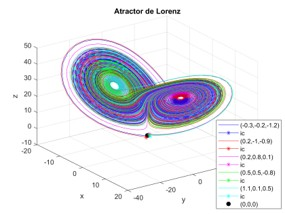
\includegraphics[width=\textwidth]{Image2.jpg}
\end{minipage}\hfill
\begin{minipage}[t]{0.49\textwidth}
  \centering
  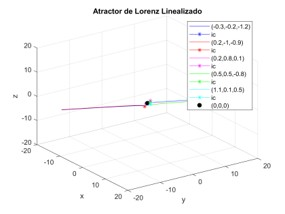
\includegraphics[width=\textwidth]{Image3.jpg}
\end{minipage}
\vspace{2pt}
\caption{Diagrama de fase del modelo de Lorentz para distintas condiciones iniciales. Modelo nolineal (derecha), modelo linealizado alrededor del punto de equilibrio (0,0,0) (izquierda).}
\end{figure}
\begin{figure}[ht]
\centering
\begin{minipage}[t]{0.49\textwidth}
  \centering
  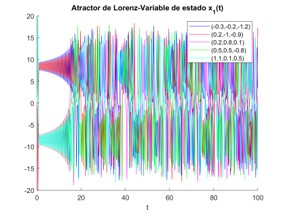
\includegraphics[width=\textwidth]{Image4.jpg}
\end{minipage}\hfill
\begin{minipage}[t]{0.49\textwidth}
  \centering
  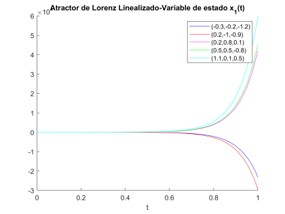
\includegraphics[width=\textwidth]{Image5.jpg}
\end{minipage}
\vspace{2pt}
\caption{Gráfico temporal de la primera variable de estado del modelo de Lorenz. Modelo nolineal (derecha), modelo linealizado alrededor del punto de equilibrio (0,0,0) (izquierda).}
\end{figure}

\section{Análisis y Discusión}
Esta sección está dedicada al analisis de los resultados.\\
En el texto deben citarse las figuras por su número, Fig. 1, Fig. 2, describiendo y comentando lo que se observa en cada una, comparando los resultados del sistema nolineal con el linealizado, la función de transferencia, etc.

\section{Conclusiones}
Incluir en esta sección una breve descripción del problema analizado, comentarios e interpretación del análisis teórico realizado sobre el modelo y de los resultados numéricos obtenidos, y una comparación de las soluciones del sistema no líneal y del linealizado.

\section{Referencias}
\begin{enumerate}
    \item Autores, Título de artículo, Revista, o Libro (año), pp.\#-\#.
    \item Autores, Título, Revista, o Libro Nro (año), pp.\#-\#.
\end{enumerate}

\end{document}
